\chapter{Building a Decision Tree \label{chapter:decisiontrees}}

{\bf Decision trees} were developed as an alternative to neural networks in the 1970s. We already saw them in Chapters~\ref{chapter:classification} and \ref{chapter:regression} as examples of supervised learning algorithms. Now we're going to get into a bit more detail about how these trees are learned from data. 

Decision trees can be adapted to solve supervised learning problems with different types of outcomes. We will focus on \textbf{classification trees} in this chapter, but the same tree building principles can be applied to solve regression problems (see Chapter~\ref{chapter:regression}). Similar modifications can also allow us to construct \textbf{survival trees}, which model survival outcomes (represented as Kaplan-Meier curves; see Chapter~\ref{chapter:km}). Decision trees can also handle count outcomes, modeling them using Poisson distributions (see Chapter~\ref{chapter:probabilitydistributions}).

%%%%%%%%%%%%%%%%%%%%%%%%%%%%%%%%%%%%%%%%%%%%%%%%%%%%%%%%%%%%%%%%%%%%%%%%%%%%%%%%%%%

\section{Example: The Wisconsin Breast Cancer Dataset \label{section:wisconsin}}

The Wisconsin breast cancer dataset\footnote{You can download the dataset from the UCI Machine Learning Repository here: \texttt{https://archive.ics.uci.edu/ml/datasets/Breast+Cancer+Wisconsin+(Diagnostic)}.} contains information about imaging features of a fine needle aspirate (FNA) of a breast mass from $569$ different subjects. Ten real-valued features are computed for each cell nucleus in the image:
{\small
\begin{enumerate}[label=(\alph*)]
\item radius (mean of distances from center to points on the perimeter)
\item texture (standard deviation of gray-scale values)
\item perimeter
\item area
\item smoothness (local variation in radius lengths)
\item compactness (perimeter$^2$ / area - 1.0)
\item concavity (severity of concave portions of the contour)
\item concave points (number of concave portions of the contour)
\item symmetry
\item fractal dimension, a statistical index of complexity quantifying how detail in a pattern changes with the scale on which it is measured
\end{enumerate}
}

The mean, standard deviation, and worst value of each feature are then computed, creating a total of $30$ features. Each image is also labeled by its true diagnosis: $B$ (for benign) or $M$ (for malignant).

Here is a decision tree for this dataset, built using the \texttt{rpart} package in R with default parameters:
\begin{center}
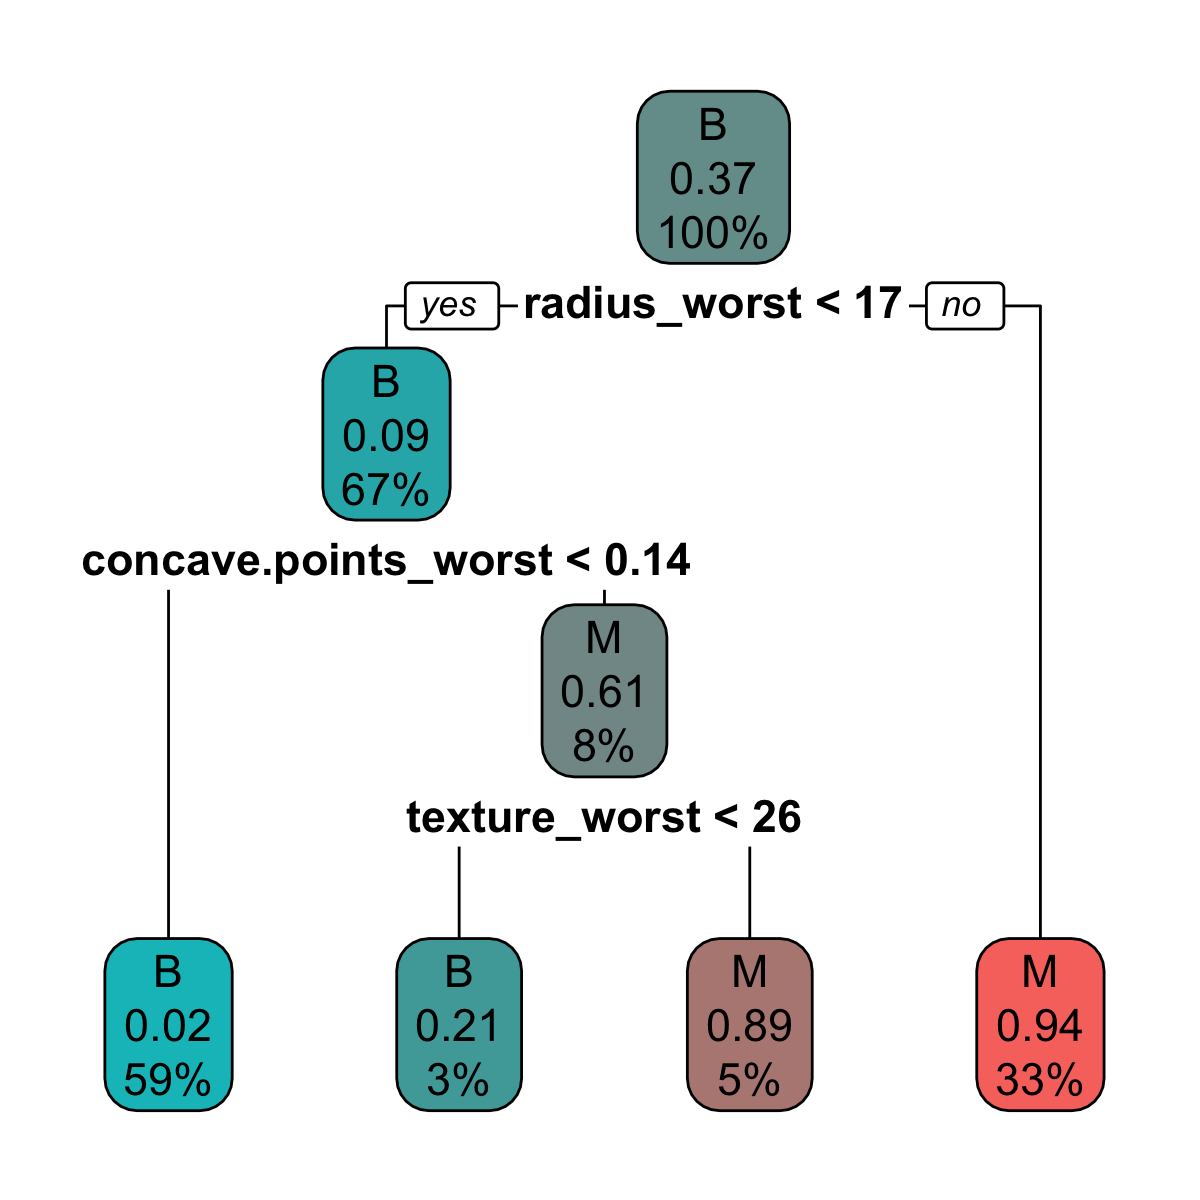
\includegraphics[width=0.7\textwidth]{img/wisconsin-decision-tree.png}
\end{center}

\begin{question}{}
What is the most important feature, as identified by the decision tree learning algorithm, for determining whether a breast mass is benign or malignant? What two other features are considered important by the tree? Which features are ignored completely?
\end{question}

\begin{question}{}
Looking at the decision tree for the Wisconsin Breast Cancer dataset, what do you think the advantages of a decision tree are for this problem over other classification methods, such as logistic regression and KNN?
\end{question}

Although there are several tree building algorithms, all of them are conceptually similar. They all try to reduce ``impurity'', or ``uncertainty'', in the outcome variable by intelligently splitting on the predictors. Trees are built recursively from root to leaves. Each internal node of the tree ``contains'' a subset of the overall dataset (this is why tree building is often called \textbf{recursive partitioning}, and why the R package is named \texttt{rpart}). At each stage, the algorithm will consider each of the existing leaf nodes and choose the split variable that maximally reduces uncertainty in the outcome. To understand how trees are built computationally, all we need to do is look at the math behind this idea. 

%%%%%%%%%%%%%%%%%%%%%%%%%%%%%%%%%%%%%%%%%%%%%%%%%%%%%%%%%%%%%%%%%%%%%%%%%%%%%%%%%%%

\section{The ID3 Algorithm}

One of the earliest approaches to building decision trees was the \textbf{ID3 algorithm}\footnote{Quinlan, J.R. ``Induction of decision trees'', Machine Learning, num. 1, pp. 81-
106, 1986.}. The ID3 Algorithm uses the concepts of entropy and information gain to build trees.

\subsection{Entropy}

\textbf{Entropy}, usually abbreviated $H$, is a measure of the uncertainty in the value of a random variable. It is the number of bits (on average) required to describe the outcome of the random variable. Here is the formula for the entropy of the discrete probability distribution governing the outcome of a random variable, $X$:
$$ H(X) = - \sum_{x} P(X = x) \log_2\left(P(X = x)\right) $$
For a Bernoulli random variable (see Chapter~\ref{chapter:probabilitydistributions}, Section~\ref{sect:bernoulli}), there are only two possible outcomes: 0 and 1. The entropy of this random variable is given by:
$$ H_\text{Bernoulli} = -\mu \log_2(\mu) - (1 - \mu) \log_2 (1 - \mu) $$
where $\mu$ is the sole parameter of the Bernoulli distribution: the probability of a positive outcome. Here is what the entropy of a Bernoulli distribution looks like as a function of $\mu$:
\begin{center}
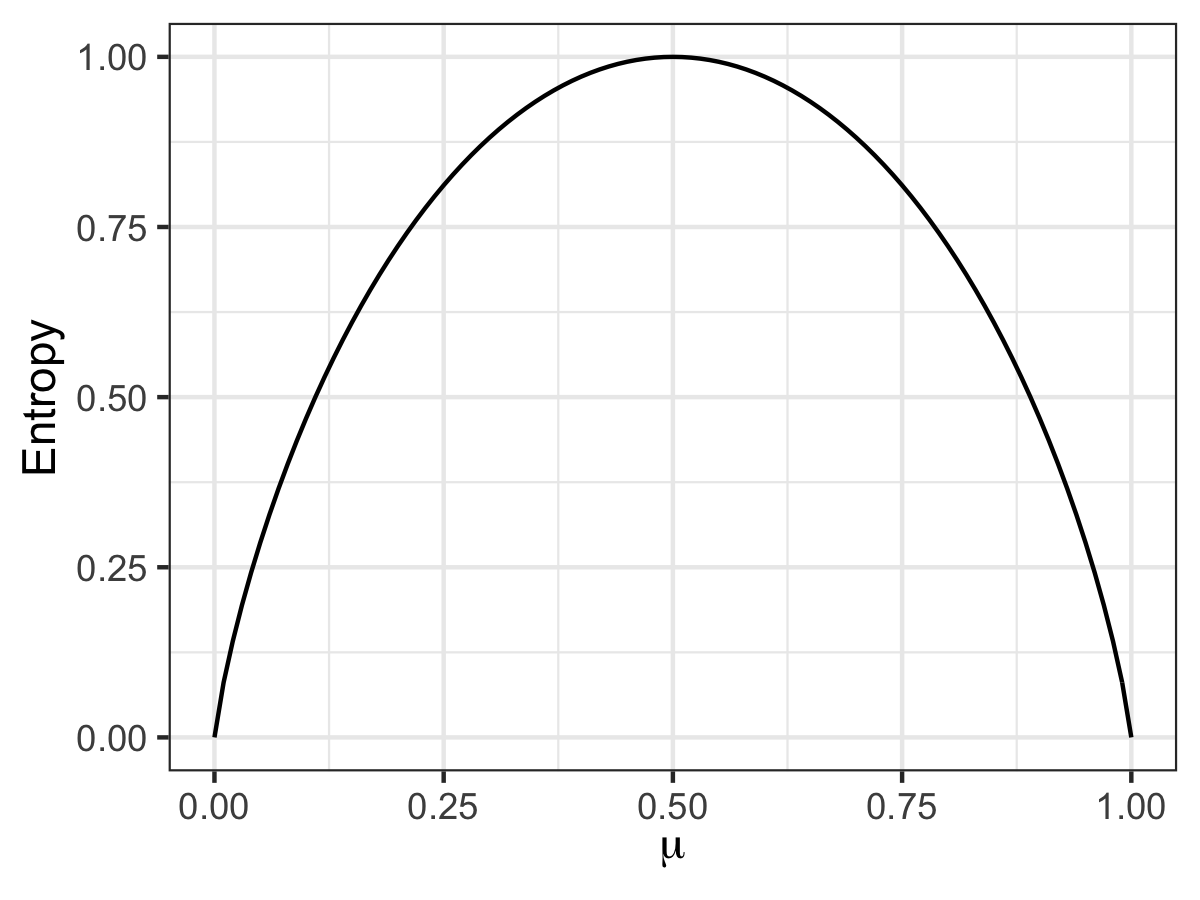
\includegraphics[width=0.7\textwidth]{img/entropy-bernoulli.png}
\end{center}

\begin{question}{}
At which value(s) of $\mu$ are we maximally uncertain about the outcome? At which value(s) of $\mu$ are we completely certain about the outcome? This should make intuitive sense if you consider the meaning of $\mu$. 
\end{question}

\subsection{Information Gain}

The goal of a decision tree is to reduce uncertainty about the outcome with every split. Let $Y$ be the outcome variable of a training set. Let $X$ be one of the predictors. \textbf{Information gain} is defined as:
\begin{align*} \text{Gain}(Y, X) &= H(Y) - \sum_{x \in \text{Values(X)}} \frac{|Y(X=x)|}{|Y|}~ H(Y(X=x)) \\
&= H(Y) - H(Y|X) \end{align*}
Since entropy is a measure of uncertainty, or impurity, in the outcome, information gain is the reduction in that uncertainty achieved by conditioning on the predictor, $X$. The tree will choose split variables for which the information gain is maximized. 
\vspace{5mm}

\begin{question}{}
Say you have a dataset where the outcome is $Y = [0, 1, 0, 1, 0, 1]$ and there are two predictors: $X = [0, 0, 1, 1, 2, 2]$, and $Z = [1, 2, 1, 2, 1, 2]$. Intuitively, which predictor would make the better splitting variable and why? Calculate $Gain(Y, X)$ and $Gain(Y, Z)$. Which value is higher?
\end{question}

\subsection{Using Entropy to Build a Decision Tree}

By understanding the concepts of entropy and information gain, we arrive naturally at the ID3 Algorithm:
\begin{enumerate}
\item Start with a single node: the root of the tree.
\item At each current leaf node:
  \begin{enumerate}
  \item Compute the information gain for each feature.
  \item Split on the one with the highest gain.
  \end{enumerate}
\item Return to Step 2. Stop when either the class distributions at all leaf nodes are entirely pure or there are no more variables left to split on.
\end{enumerate}

%%%%%%%%%%%%%%%%%%%%%%%%%%%%%%%%%%%%%%%%%%%%%%%%%%%%%%%%%%%%%%%%%%%%%%%%%%%%%%%%%%%

\section{Example: Happiness Dataset}

Let's build a decision tree for a simple example, using the ID3 algorithm. Assume we surveyed 10 people and asked them whether they were happy or unhappy. We also asked whether they had friends (yes/no), money (poor/enough/rich), and free time (none/some). The data look like this:

{\small
\begin{center}
\begin{tabular}{ccccc}
\toprule
Datapoint ID & friends $(X_1)$ & money $(X_2)$ & free time $(X_3)$ & happy $(Y)$ \\
\midrule
1 & 1 & 1 & 0 & 0 \\
2 & 1 & 1 & 1 & 0 \\
3 & 0 & 1 & 1 & 0 \\
4 & 0 & 0 & 0 & 0 \\
5 & 1 & 0 & 0 & 0 \\
6 & 0 & 0 & 0 & 0 \\
\midrule
7 & 1 & 2 & 1 & 1 \\
8 & 1 & 0 & 1 & 1 \\
9 & 0 & 0 & 1 & 1 \\
10 & 1 & 0 & 0 & 1 \\
\bottomrule
\end{tabular}

\begin{align*}
	x_1 = \left\{ \begin{array}{cc} 0 & \text{no friends} \\ 1 & \text{friends} \end{array} \right.
	\qquad
	x_2 = \left\{ \begin{array}{cc} 0 & \text{poor} \\ 1 & \text{enough money} \\ 2 & \text{rich} \end{array} \right.
	\qquad
	x_3 = \left\{ \begin{array}{cc} 0 & \text{no free time} \\ 1 & \text{some free time} \end{array} \right.
\end{align*}
\end{center}
}

\begin{question}{}
Build a decision tree for this dataset using the ID3 algorithm. To get started, you need to know the entropy of the overall outcome distribution. It is:
$$ H(Y) = - \frac{4}{10} \log_2 \frac{4}{10} - \frac{6}{10} \log_2 \frac{6}{10} = \textbf{0.971} $$
We will go through the calculations below. As we go, you can start to draw the tree on another page.
\begin{enumerate}
\item[(a)] Perform the initial split at the tree root to determine which variable to split on first. Update the tree with this information.

\begin{align*}
\frac{|Y(X_1 = 0)|}{|Y|} H[Y(X_1 = 0)] &= \hspace{0.5\textwidth}\\[2mm]
\frac{|Y(X_1 = 1)|}{|Y|} H[Y(X_1 = 1)] &= \\[2mm]
\text{Gain}(Y, X_1) &= \\[2mm]
\frac{|Y(X_2 = 0)|}{|Y|} H[Y(X_2 = 0)] &= \\[2mm]
\frac{|Y(X_2 = 1)|}{|Y|} H[Y(X_2 = 1)] &= \\[2mm]
\frac{|Y(X_2 = 2)|}{|Y|} H[Y(X_2 = 2)] &= \\[2mm]
\text{Gain}(Y, X_2) &= \\[2mm]
\frac{|Y(X_3 = 0)|}{|Y|} H[Y(X_3 = 0)] &= \\[2mm]
\frac{|Y(X_3 = 1)|}{|Y|} H[Y(X_3 = 1)] &= \\[2mm]
\text{Gain}(Y, X_3) &= 
\end{align*}

\item[(b)] We see that two of the leaves of our tree are ``pure'', meaning that all of the training examples that arrive there are of one outcome class. For those two leaves, we're done. However, for the third ($X_2 = 0$, or poor), we need to perform another split. Perform the split at the $X_2=0$ node to find which variable to split on next and update the tree with this information. 

\begin{align*}
H[Y(X_2 = 0)] &= \\[2mm]
\frac{|Y(X_2 = 0, X_1 = 0)|}{|Y(X_2=0)|} H[Y(X_2 = 0, X_1 = 0)] &= \hspace{0.5\textwidth}\\[2mm]
\frac{|Y(X_2 = 0, X_1 = 1)|}{|Y(X_2=0)|} H[Y(X_2 = 0, X_1 = 1)] &= \hspace{0.5\textwidth}\\[2mm]
\text{Gain}(Y(X_2=0), X_1) &= \\[2mm]
\frac{|Y(X_2 = 0, X_3 = 0)|}{|Y(X_2=0)|} H[Y(X_2 = 0, X_3 = 0)] &= \hspace{0.5\textwidth}\\[2mm]
\frac{|Y(X_2 = 0, X_3 = 1)|}{|Y(X_2=0)|} H[Y(X_2 = 0, X_3 = 1)] &= \hspace{0.5\textwidth}\\[2mm]
\text{Gain}(Y(X_2=0), X_3) &= \\[2mm]
\end{align*}

\item[(c)] We need to do one more split on the $X_2 = 0, X_3 = 0$ node. The only variable left to split on is $X_1$ (friends). Perform this split and add this information to the tree. 
\end{enumerate}
\end{question}

%%%%%%%%%%%%%%%%%%%%%%%%%%%%%%%%%%%%%%%%%%%%%%%%%%%%%%%%%%%%%%%%%%%%%%%%%%%%%%%%%%%

\section{Alternative Splitting Criteria}

Information gain is not the only criterion that is used in decision tree algorithms. In fact, the tree built for the Wisconsin Breast Cancer dataset in Section~\ref{section:wisconsin} used a different criterion, the mean decrease in Gini impurity, or \textbf{Gini index}, because it is the default in R's \texttt{rpart} package. 

The Gini impurity measures how often a randomly chosen element from a set would be incorrectly labeled if it were randomly labeled using the distribution of labels in the subset. It sums up the probability of an item with label $i$ being chosen ($p_i$) multiplied by the probability $\sum_{j \neq i} p_j = 1 - p_i$ that a mistake is made in classifying it. The formula is:
$$ G(p) = \sum_{i} p_i (1 - p_i) = 1 - \sum_i p_i^2 $$
which for a Bernoulli distribution is 
$$ G_\text{Bernoulli} = 1 - \mu^2 - (1-\mu)^2. $$
The Gini impurity plays a role analogous to entropy. The Gini index is a weighted sum of the Gini impurities within the children of a particular split; if it is low, it means the split was successful in reducing impurity. 

\vspace{3mm}

\begin{question}{}
Plots of the Gini impurity vs. entropy for a Bernoulli distribution are shown below. What do you notice about the value(s) of $\mu$ for which each is maximized or minimized?
\begin{center}
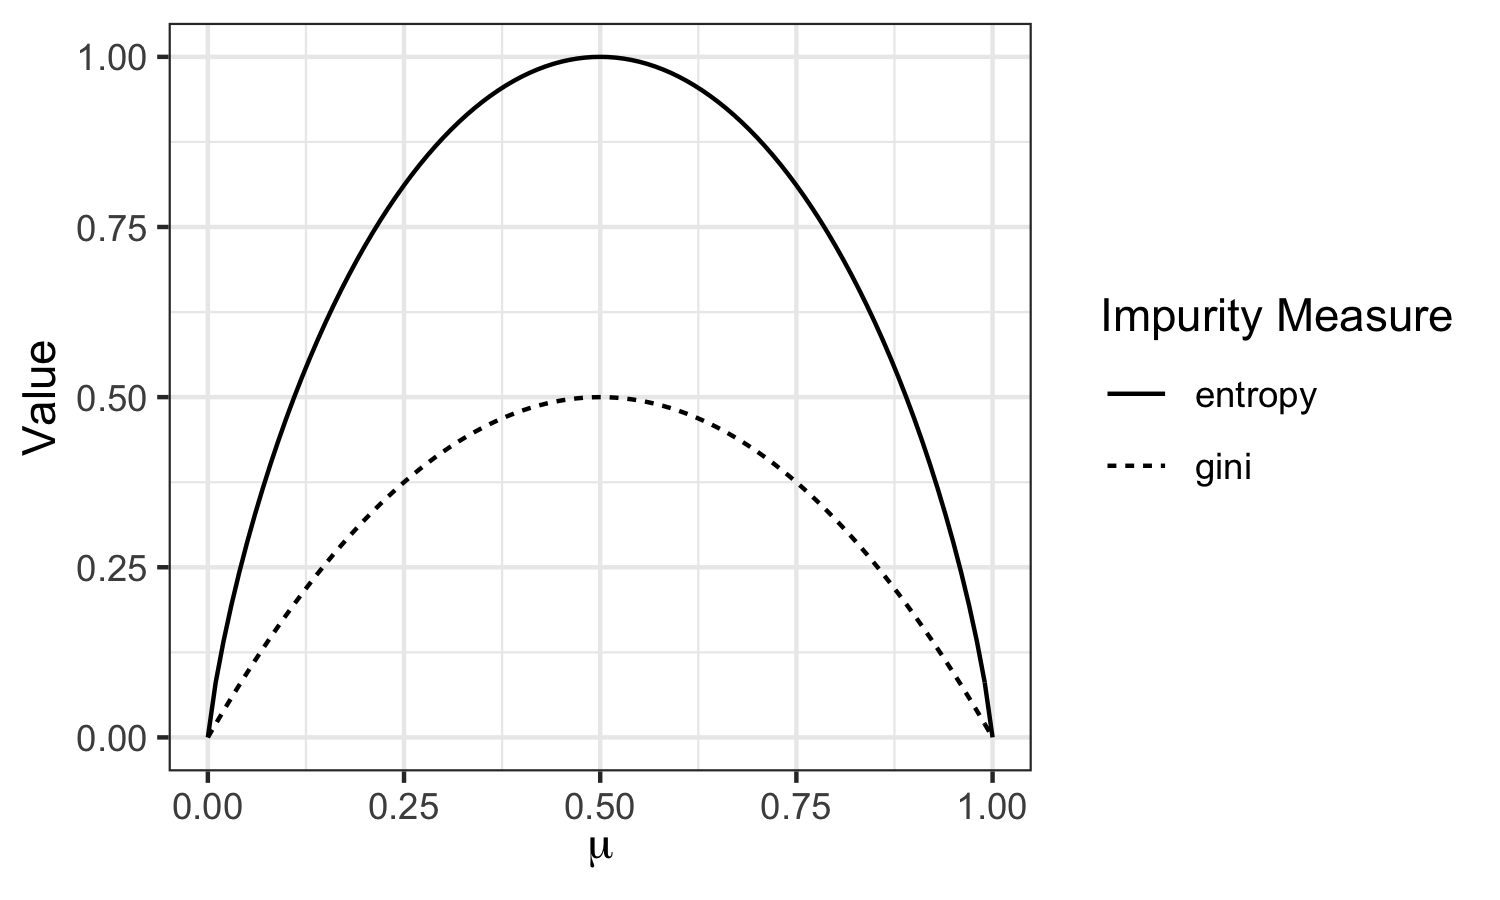
\includegraphics[width=0.8\textwidth]{img/comparison-entropy-gini-bernoulli.png}
\end{center}
\end{question}

Entropy and Gini impurity are similar and usually, though not always, yield similar trees. The Gini impurity is computationally faster because it does not make use of logarithms as the entropy does. This can make a difference as the number of features grows. 

%%%%%%%%%%%%%%%%%%%%%%%%%%%%%%%%%%%%%%%%%%%%%%%%%%%%%%%%%%%%%%%%%%%%%%%%%%%%%%%%%%%

\section{Decision Tree Regression}

So far we've assumed that our outcome is discrete. But what happens if it's numeric? (That is, what if we want to perform regression instead of classification?)

In that case, we use \textbf{standard deviation reduction} instead of information gain to decide which variables to split on. The sample standard deviation of an outcome, $y$, is defined as:
$$ S(Y) = \sqrt{\frac{\sum_i(y^{(i)} - \overline{y})}{n-1}} $$
The procedure is identical to the ID3 algorithm except that it uses conditional standard deviation instead of information gain to decide on features. We define
$$ S(Y, X) = \sum_{x} P(X = x)~ S(Y(X=x)) $$
and at each current leaf node, we split on the variable where the reduction in standard deviation, $S(Y) - S(Y,X)$, is the highest. 
\vspace{2mm}

\begin{question}{}
Imagine you have a dataset with two predictors, $x_1$ and $x_2$, each of which is binary (can only be 0 or 1). Here are the distributions of outcome values associated with $x_1$ and $x_2$:
\begin{center}
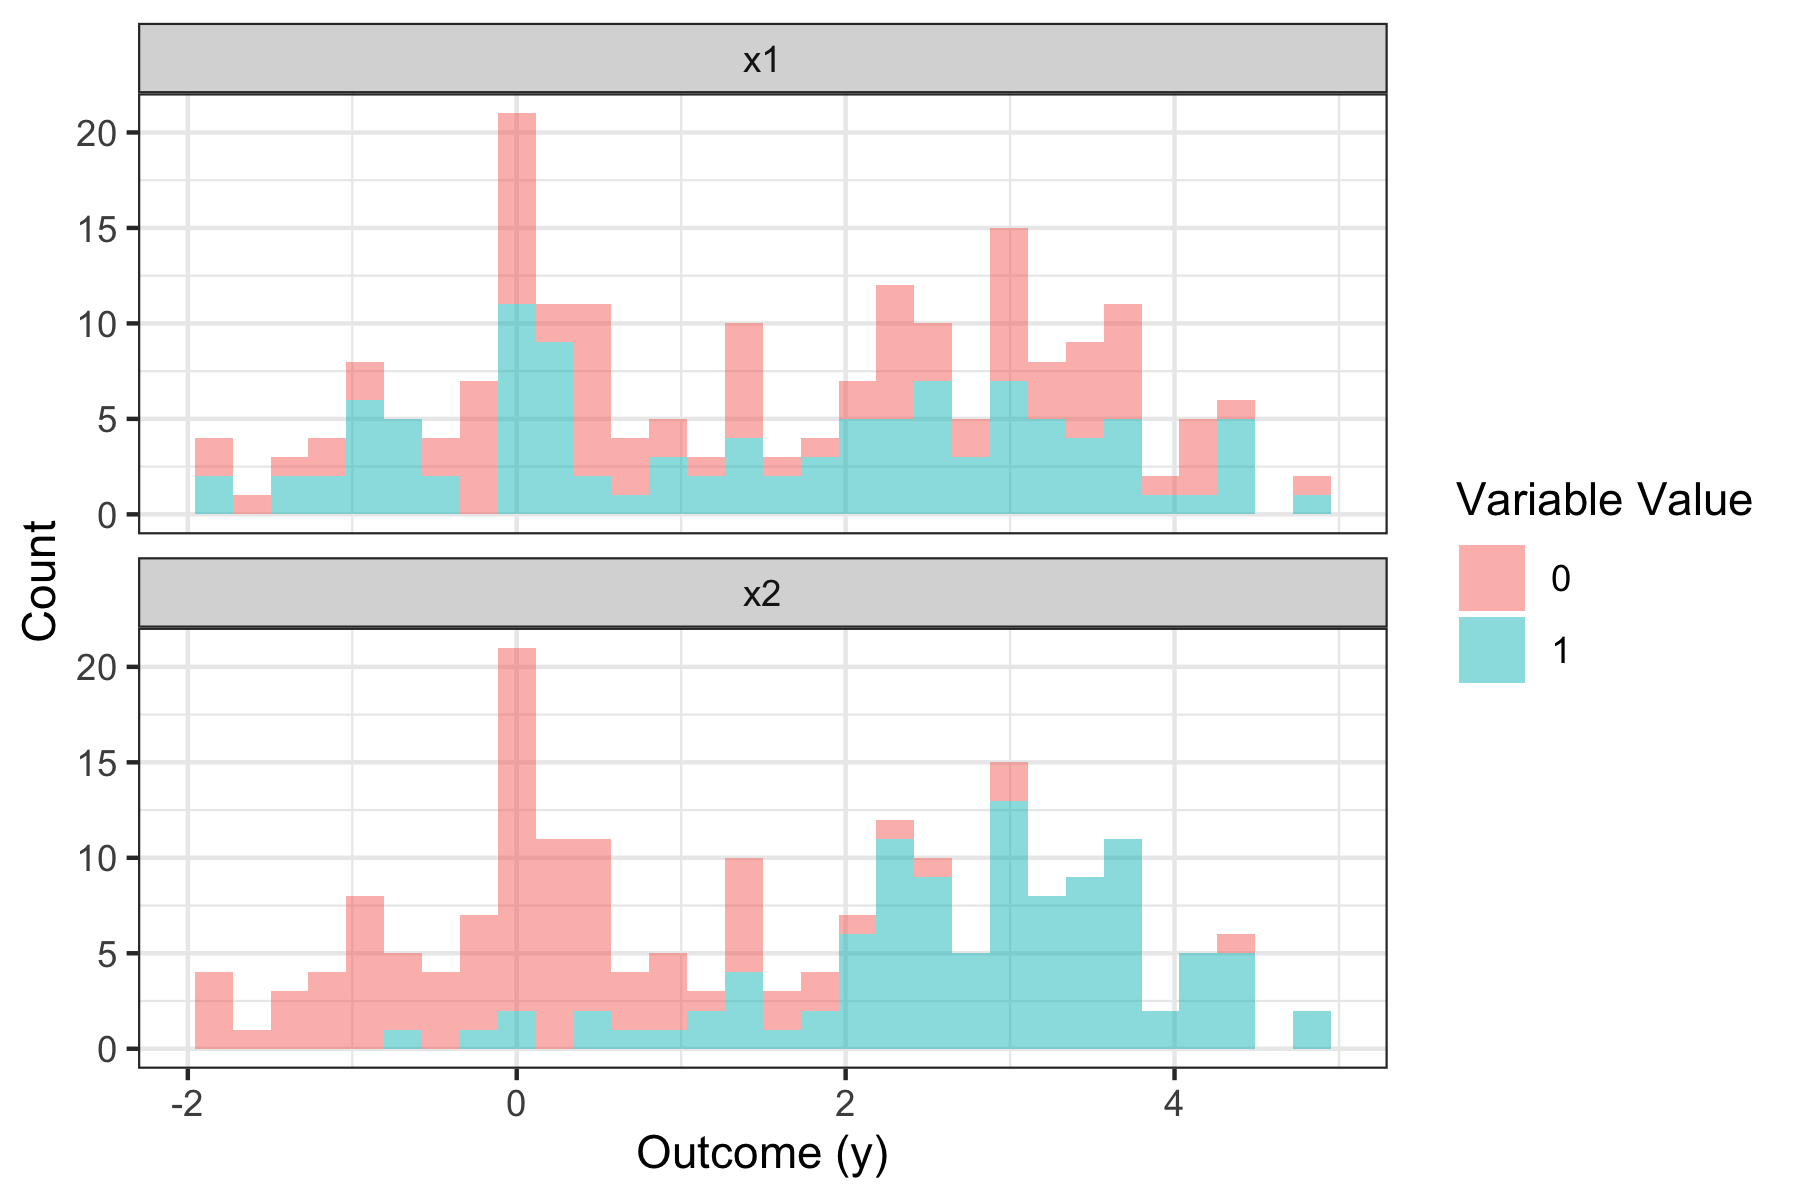
\includegraphics[width=0.7\textwidth]{img/esl-reg-decision-tree-varsplit.png}
\end{center}
Based on the idea of standard deviation reduction, which of these two variables, $x_1$ or $x_2$, would make the most sense for a decision tree to split on? What would such a split look like and what would the output value of the tree (the predicted value of $y$) be for each side of the split?
\end{question}

%%%%%%%%%%%%%%%%%%%%%%%%%%%%%%%%%%%%%%%%%%%%%%%%%%%%%%%%%%%%%%%%%%%%%%%%%%%%%%%%%%%

\section{Numeric Predictors}

Although the Happiness Dataset contained only discrete predictors, decision trees can also handle numeric predictors. We've seen this already with the Wisconsin Breast Cancer dataset. 

There are different strategies for deciding on an optimal split for a predictor. The most common approach is to consider all possible splits. So for example, if a predictor has values $10, 11, 16, 18, 20$, and $35$, the tree building algorithm would consider all $N-1 = 5$ possible split points. If a dataset has a large number of numeric features or features with lots of different possible values, therefore, it can really slow down the construction of the tree.
\vspace{5mm}

\begin{question}{}
Here are histograms of $10$ of the predictors in the Wisconsin Breast Cancer dataset. Only the ``worst'' variable version of each predictor is shown for clarity. Which variable, and which threshold, appears to show the clearest division of samples into $B$ and $M$ groups? Compare your choice to the first split of the tree in Section~\ref{section:wisconsin}. 
\begin{center}
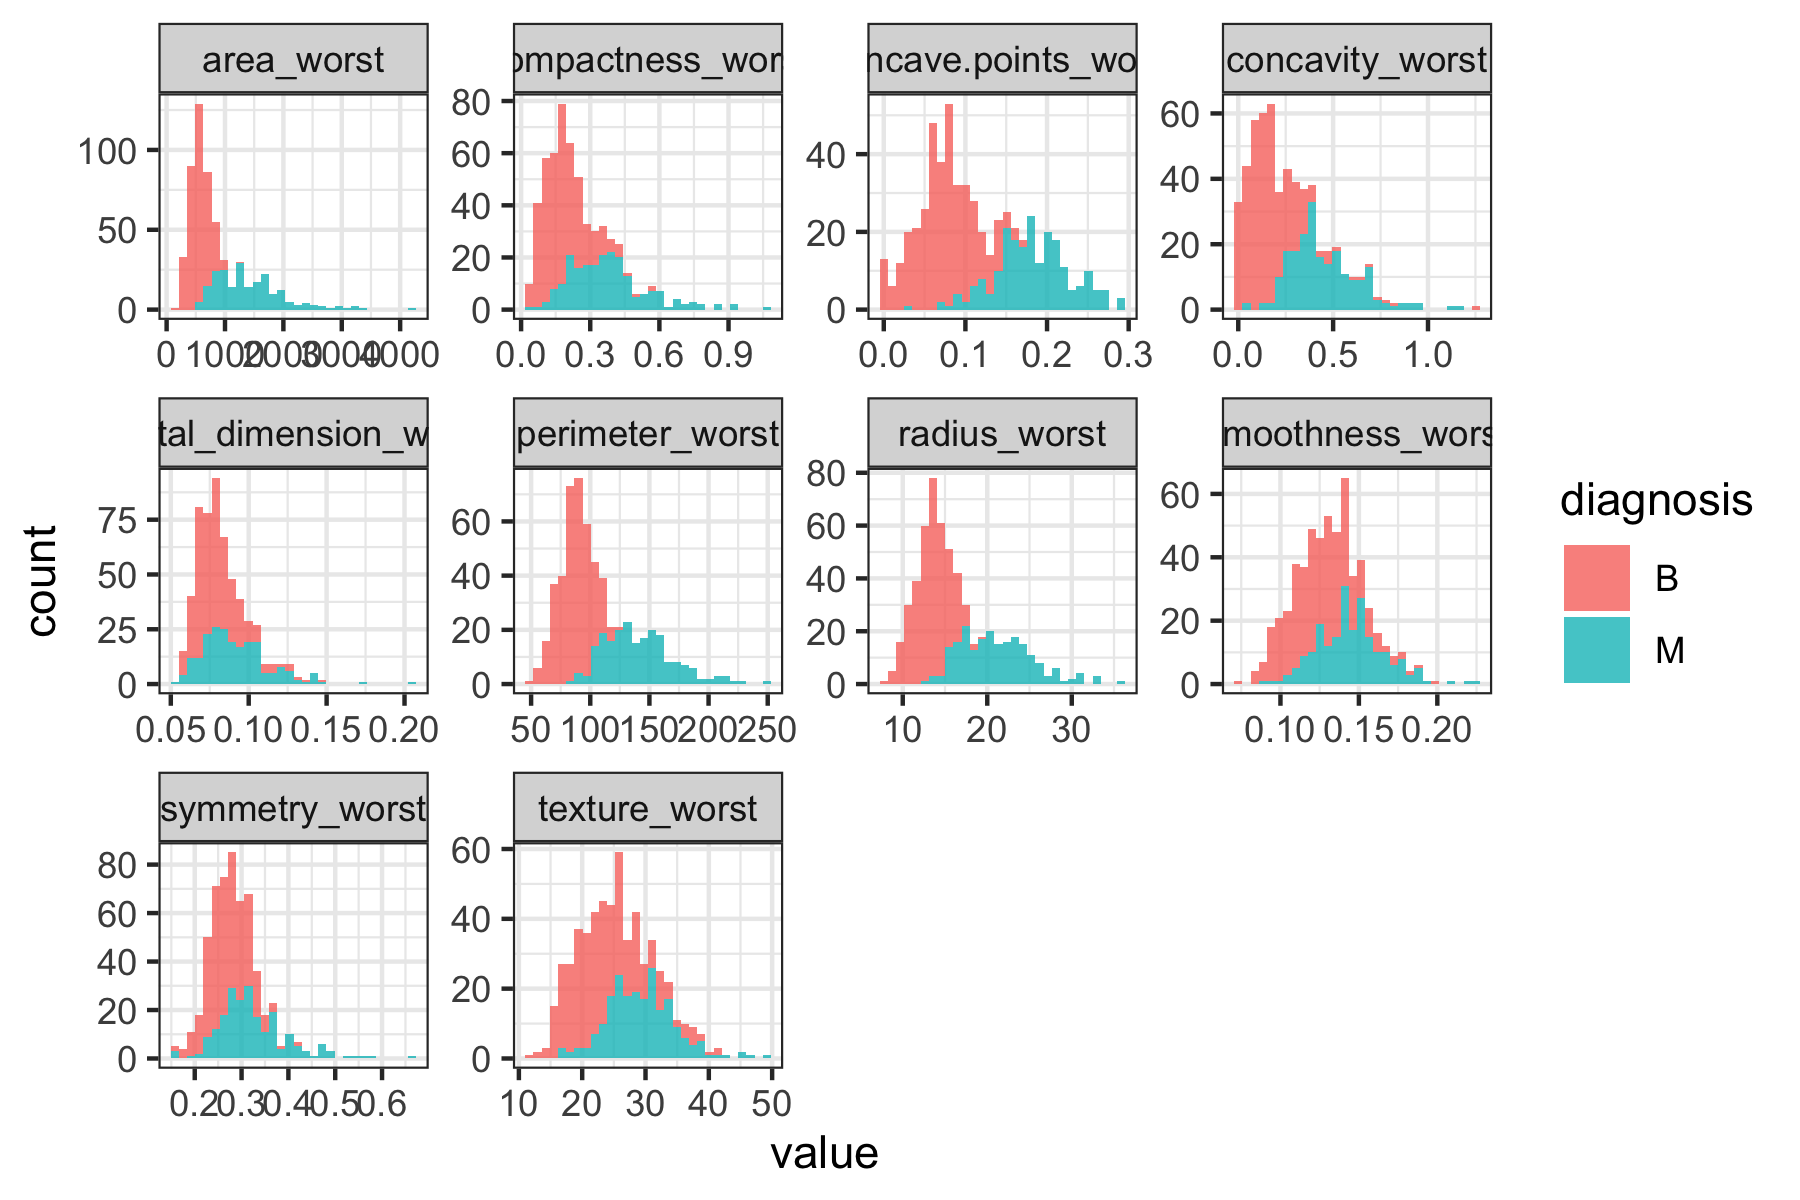
\includegraphics[width=\textwidth]{img/wisconsin-variable-plots.png}
\end{center}
\end{question}

